\appendix
\chapter{Implementation}
\section{Logo Activity}
\begin{figure}[h!]
	\centering
	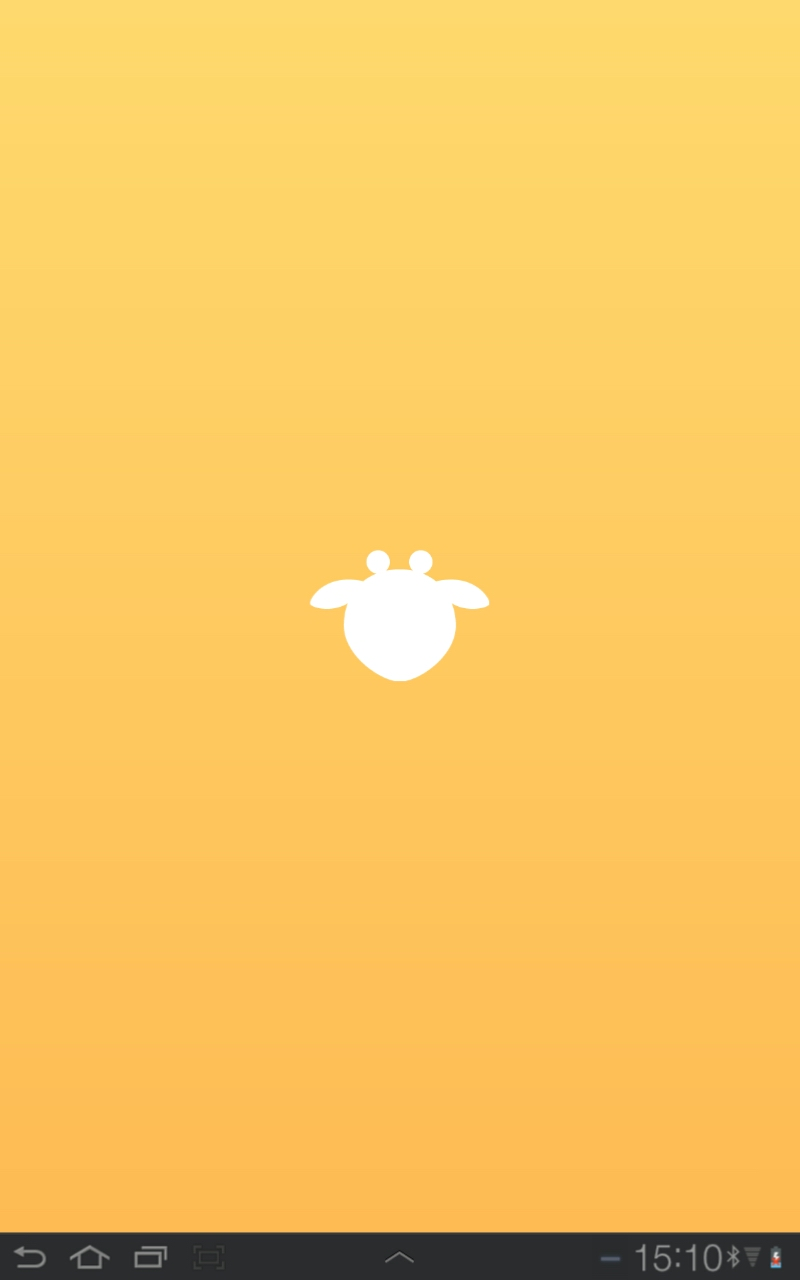
\includegraphics[scale=0.3]{gfx/logo-activity_1.jpg}
	\caption{LogoActivity in portrait mode}
	\label{fig:logo-activity_1}
\end{figure}

\begin{figure}[h!]
	\centering
	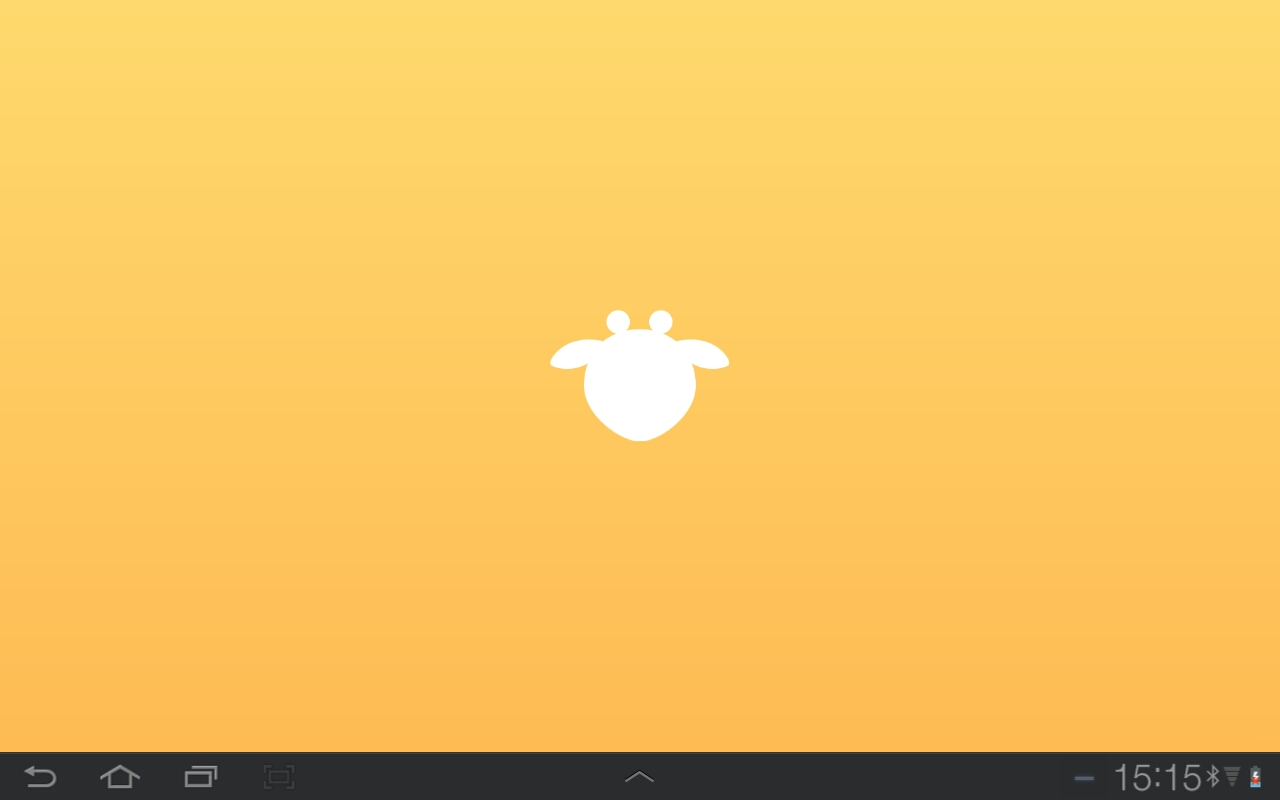
\includegraphics[scale=0.3]{gfx/logo-activity_2.jpg}
	\caption{LogoActivity in landscape mode}
	\label{fig:logo-activity_2}
\end{figure}

\section{Profile select activity}
\begin{figure}[h!]
	\centering
	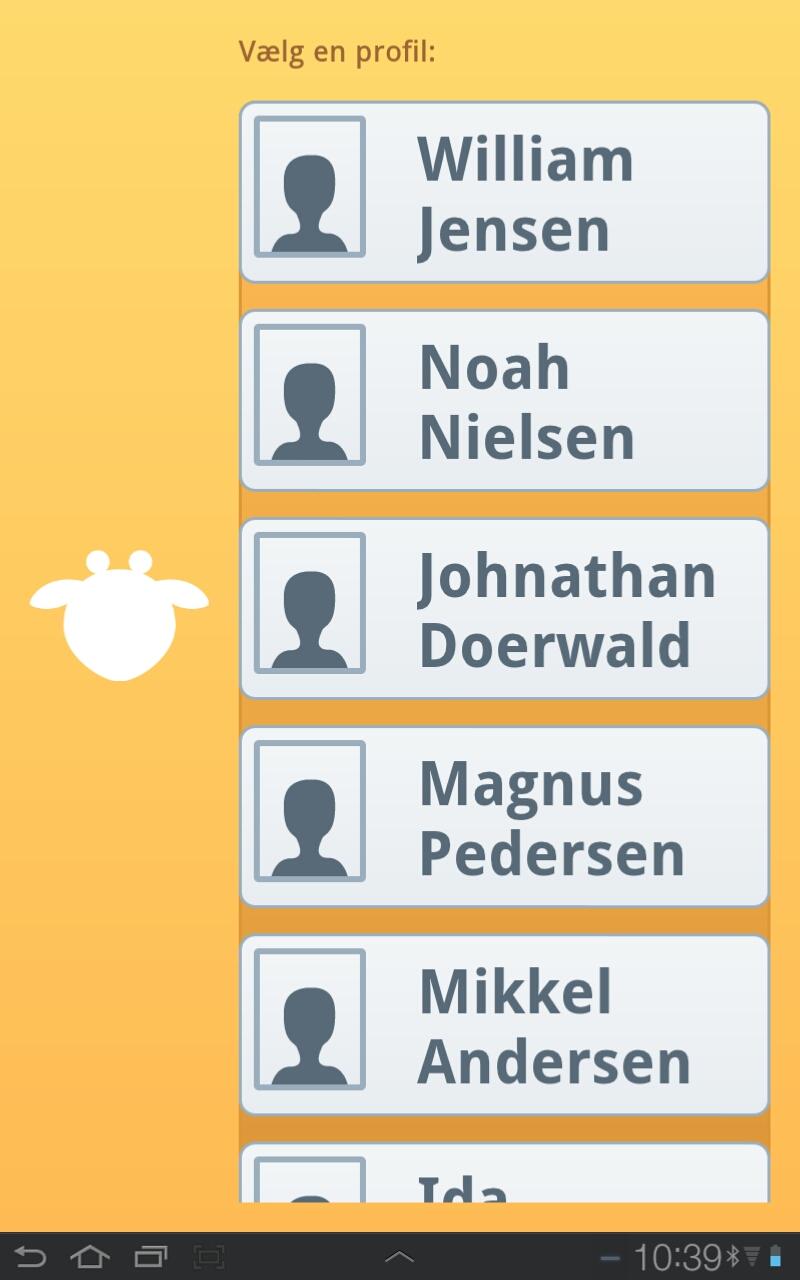
\includegraphics[scale=0.3]{gfx/profile-select-activity_1.jpg}
	\caption{ProfileSelectActivity in portrait mode}
	\label{fig:profile-select-activity_1}
\end{figure}

\chapter{Use Cases}
\label{appendix_use_cases}

\section{New Guardian Log in}
Karen is new at her workplace where she has had her GIRAF profile created already and is now trying to use a GIRAF tablet for the first time. 
She has recieved her authentication QR-code, and after she has booted the tablet up, it prompts her to scan her QR-code. 
She presses accept and is sent to the QR-code app, where she scans her code and is sent back to the GIRAF system after it has scanned her code. 
She is now in guardian mode and can access the children she has been authorized for.

\section{Configuring an app for a child}
The GIRAF systems where Karen works have recently received a new app that she wants to use with one of the kids. 
To prepare, she has the tablet she is logged in on and wants to open the settings app to personalize the app ahead. 
When she opens the app, she is given a list of profiles where she chooses the profile for the child. 

The settings app then becomes active, and displays a list of all apps that are available to the child, and the bottom the app has a button for adding more apps to the list. 
She presses that button and receives a list of all available apps on the system. 
She then finds the new app, selects it and confirms that she wishes to make this app available to this child.
She is then sent back into the settings app with the list of apps where she can now choose the new app. 
She does so, and the settings app opens a page next to the list where she is asked to change settings in ``text'' mode or in snapshot mode. 

She first chooses ``text'' mode, and receives a list of the settings she can change in the app. 
She wants to change the background color of the app, so she finds the setting labelled ``Baggrund'', presses it and is given the option of choosing a picture or a color as background. 
She selects color and is given the option of choosing the color from a color wheel. 
She marks the desired color and presses ``OK'' (which means her new settings have been saved). 

She wants to change other aspects of the app as well, but prefers doing so in snapshot mode, so in the list of apps available to the child, she presses the app again, and now selects snapshot mode when prompted.
An interactive snapshot of the given app is now opened next to the list of apps, and pressing elements of the app allows her to configure them. 
She presses an element she would like to resize and does a pinching motion to make the element smaller. 
She then presses the ``OK'' button (which means her settings have been saved) at the bottom of the screen and is returned to the interactive snapshot's starting state.
She is finished editting the settings of the app and so she presses the Home button and is returned to her launcher.

\section{Launching an app for a child in Guardian mode}
Karen is trying to work with a child and wants to open an app with that child's profile. 
In guardian mode, she presses the icon for the given app and receives a list of profiles to launch the app with. 
The child's profile is not directly visible, so she scrolls down the list until she finds the correct profile. 
She selects the profile and the app then launches with the settings specified for that profile.

\section{Letting a child use an app for a limited time}
Karen wants to let a child use an app in the child's break. 
With the system in guardian mode, she presses the icon for the app. 
A list of profiles then pops up, and by swyping in from the left, a list of apps that can interact with the app becomes visible. 
With a time app installed, it is visible on the list and allows Karen to choose a period of time where the app it is used with will become unavailable after this time runs out.

\chapter{QR-codes}
\section{QR-code test}
\begin{figure}[h!]
	\centering
	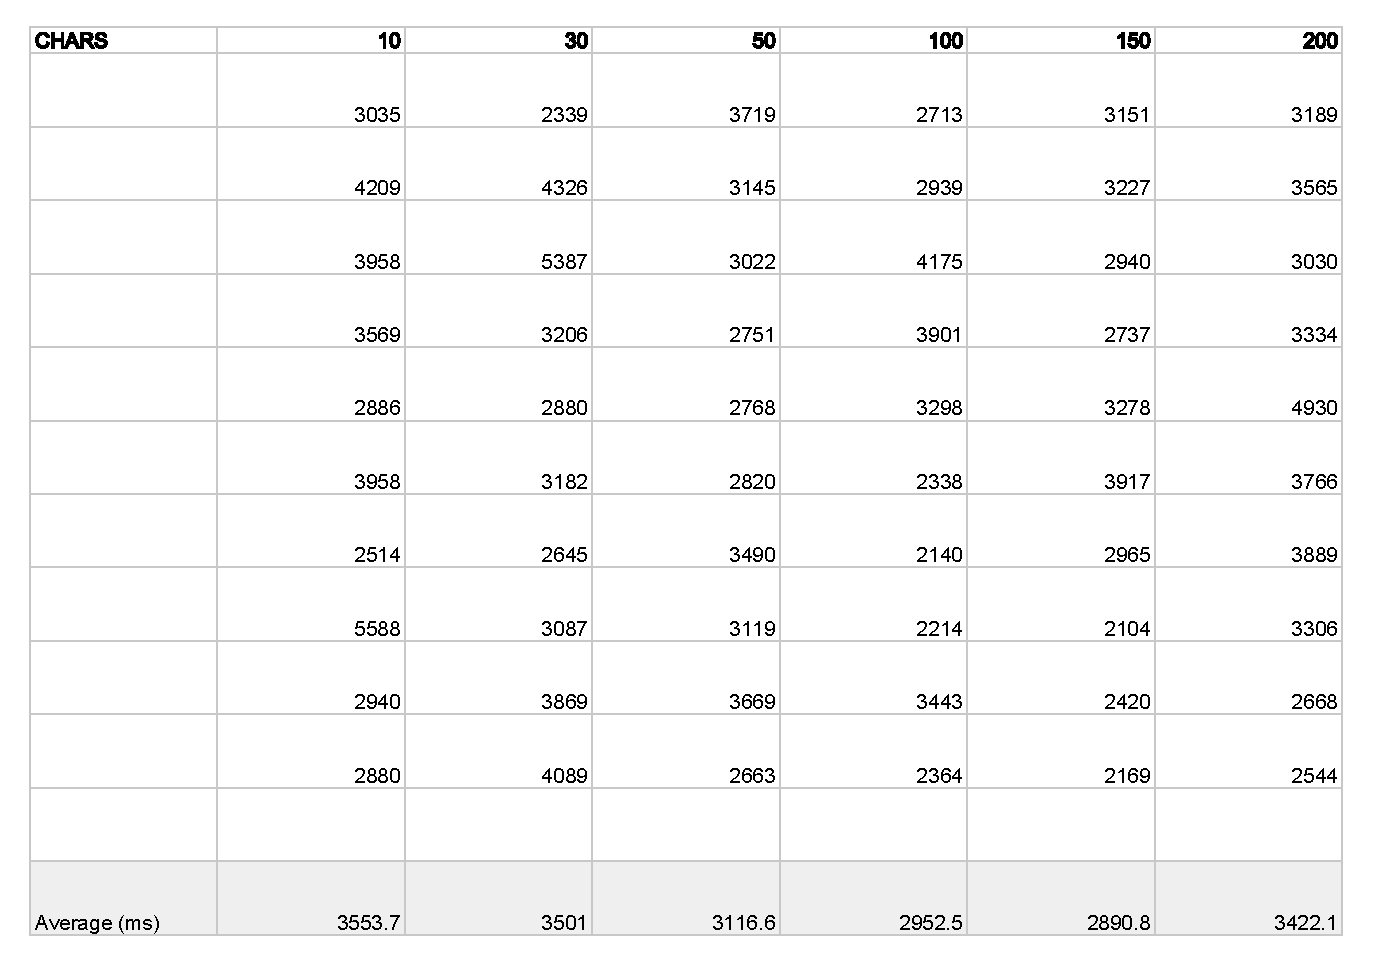
\includegraphics[scale=0.6]{gfx/QR-test.pdf}
	\caption{The results from the QR-code test, all times are in ms.}
	\label{fig:QR-code-test}
\end{figure}

\chapter{Usability Test}
\label{usability_test}
\section{Test Invitation}
\begin{figure}[h!]
	\centering
	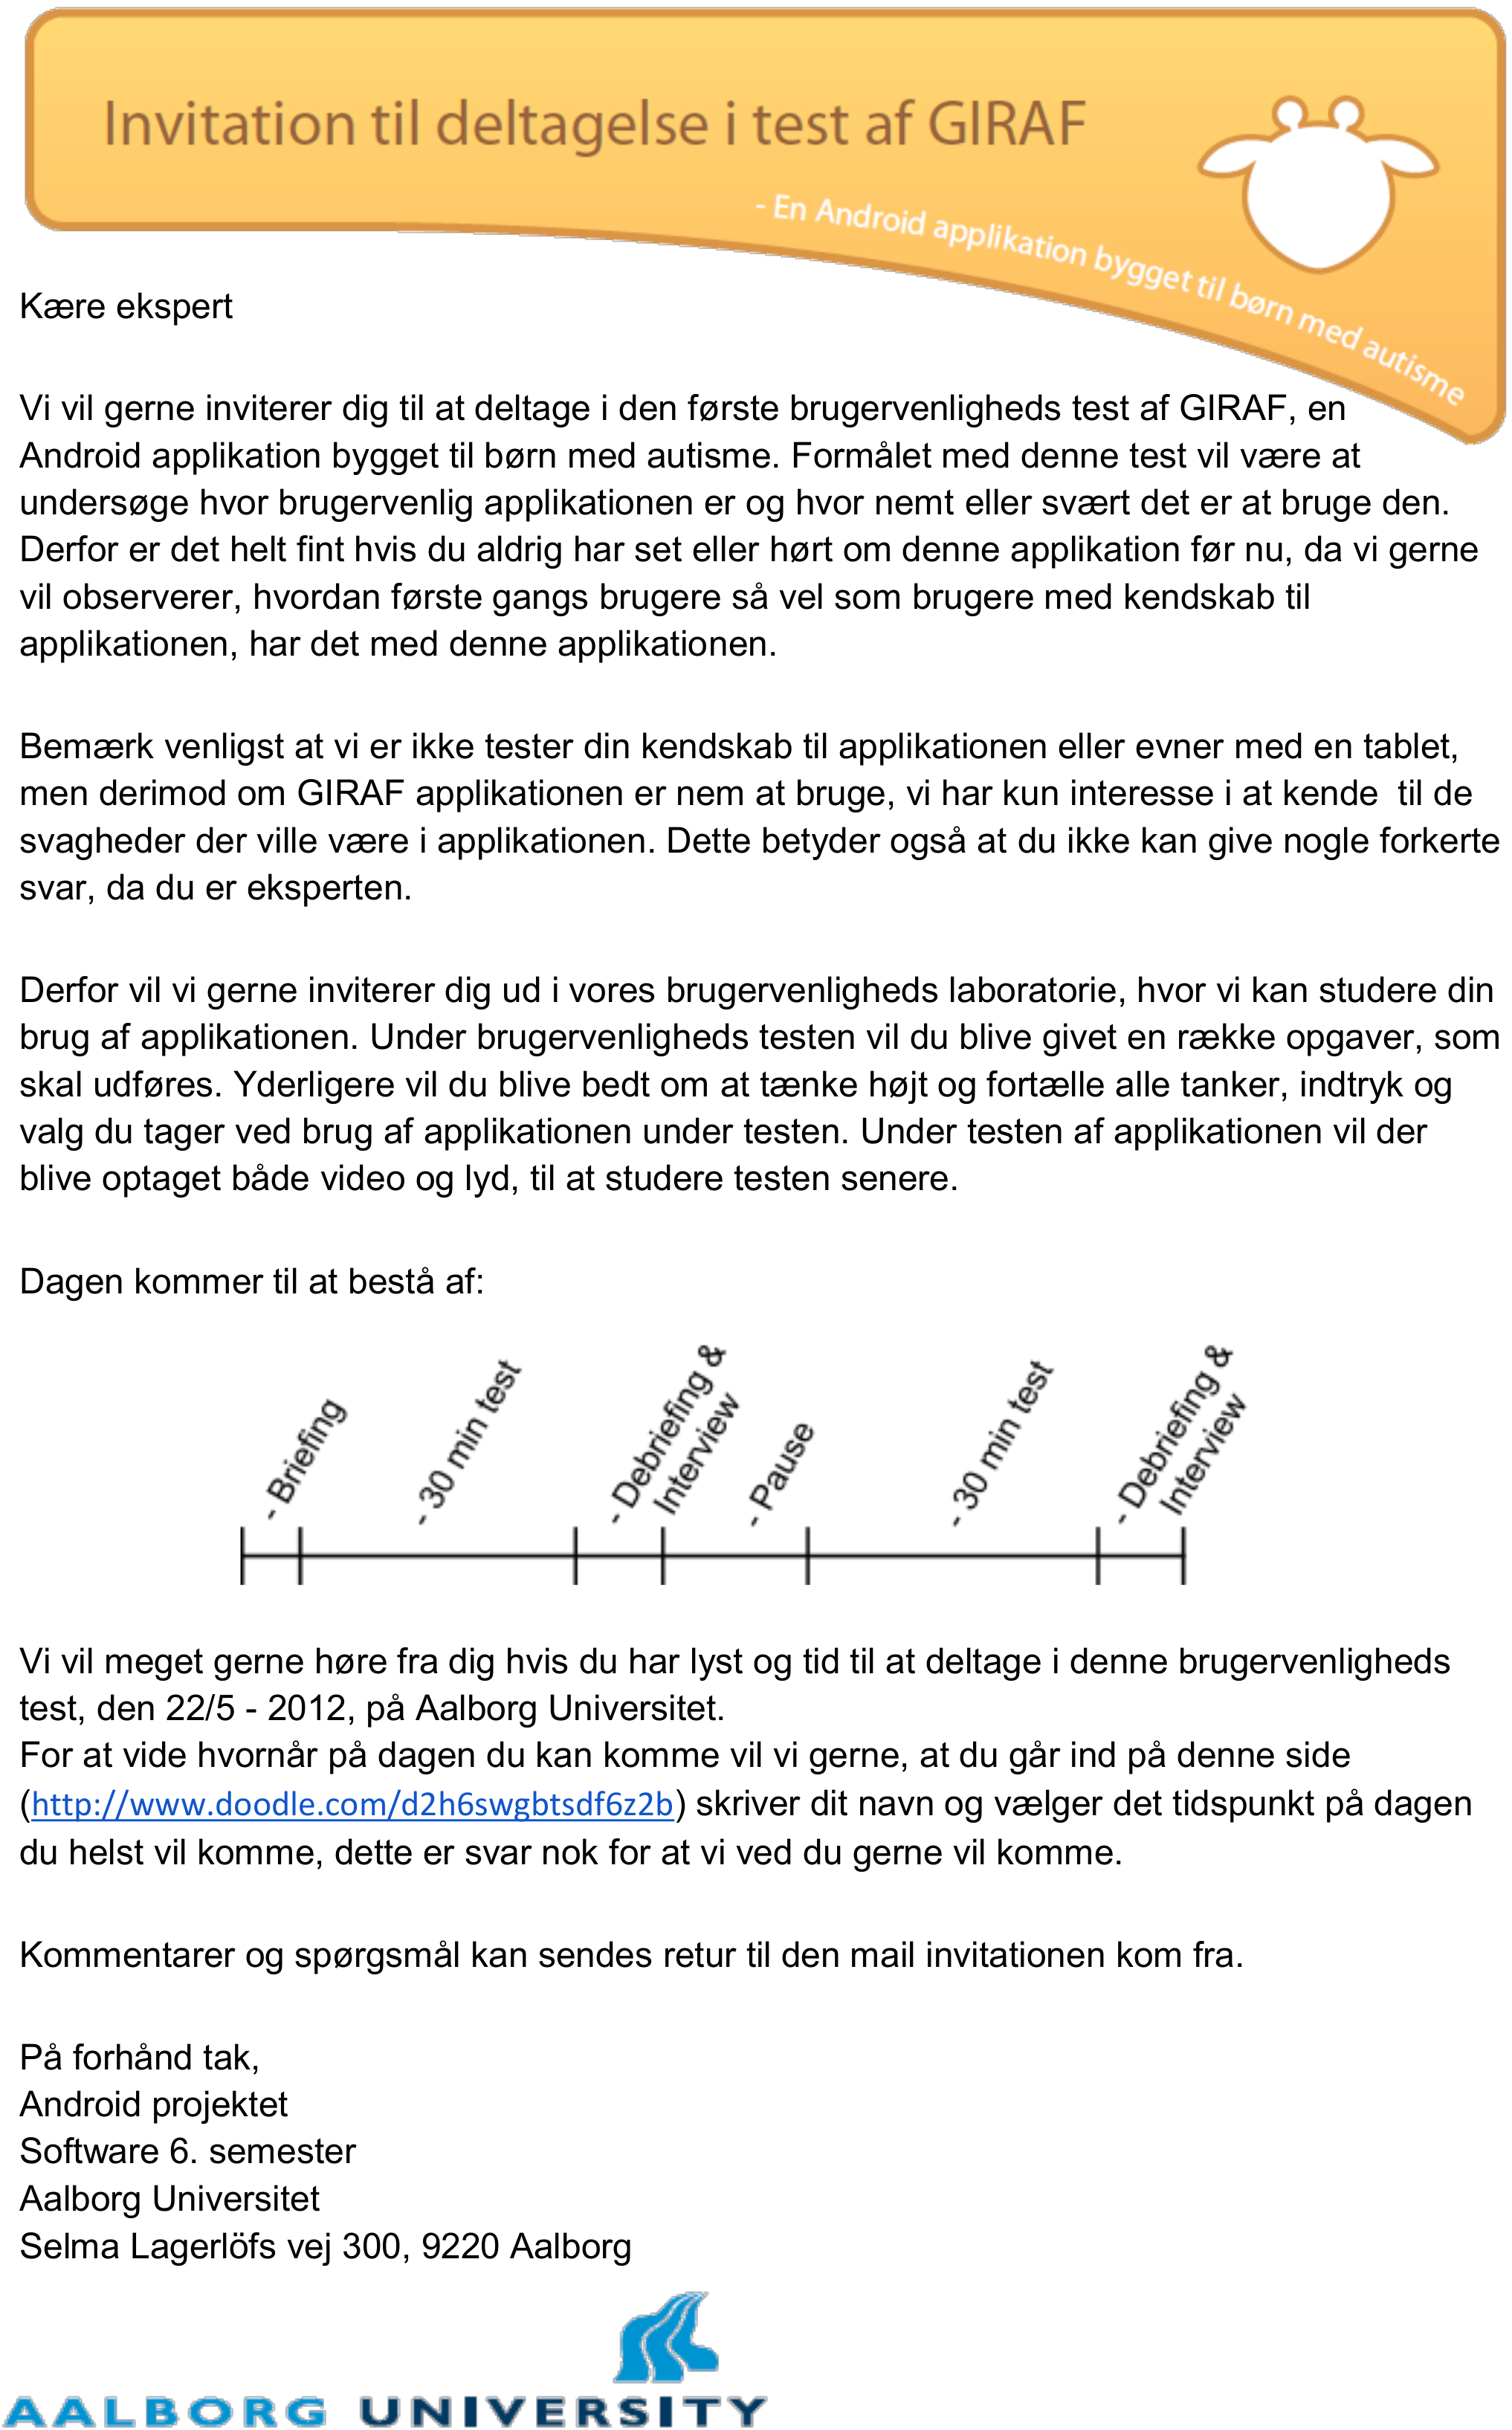
\includegraphics[scale=0.65]{gfx/usabilitytest-invitation.png}
	\caption{Invitation asking for customer participation in a usability test}
	\label{fig:usability_invitation}
\end{figure}

\section{Test Briefing}
\begin{figure}[h!]
	\centering
	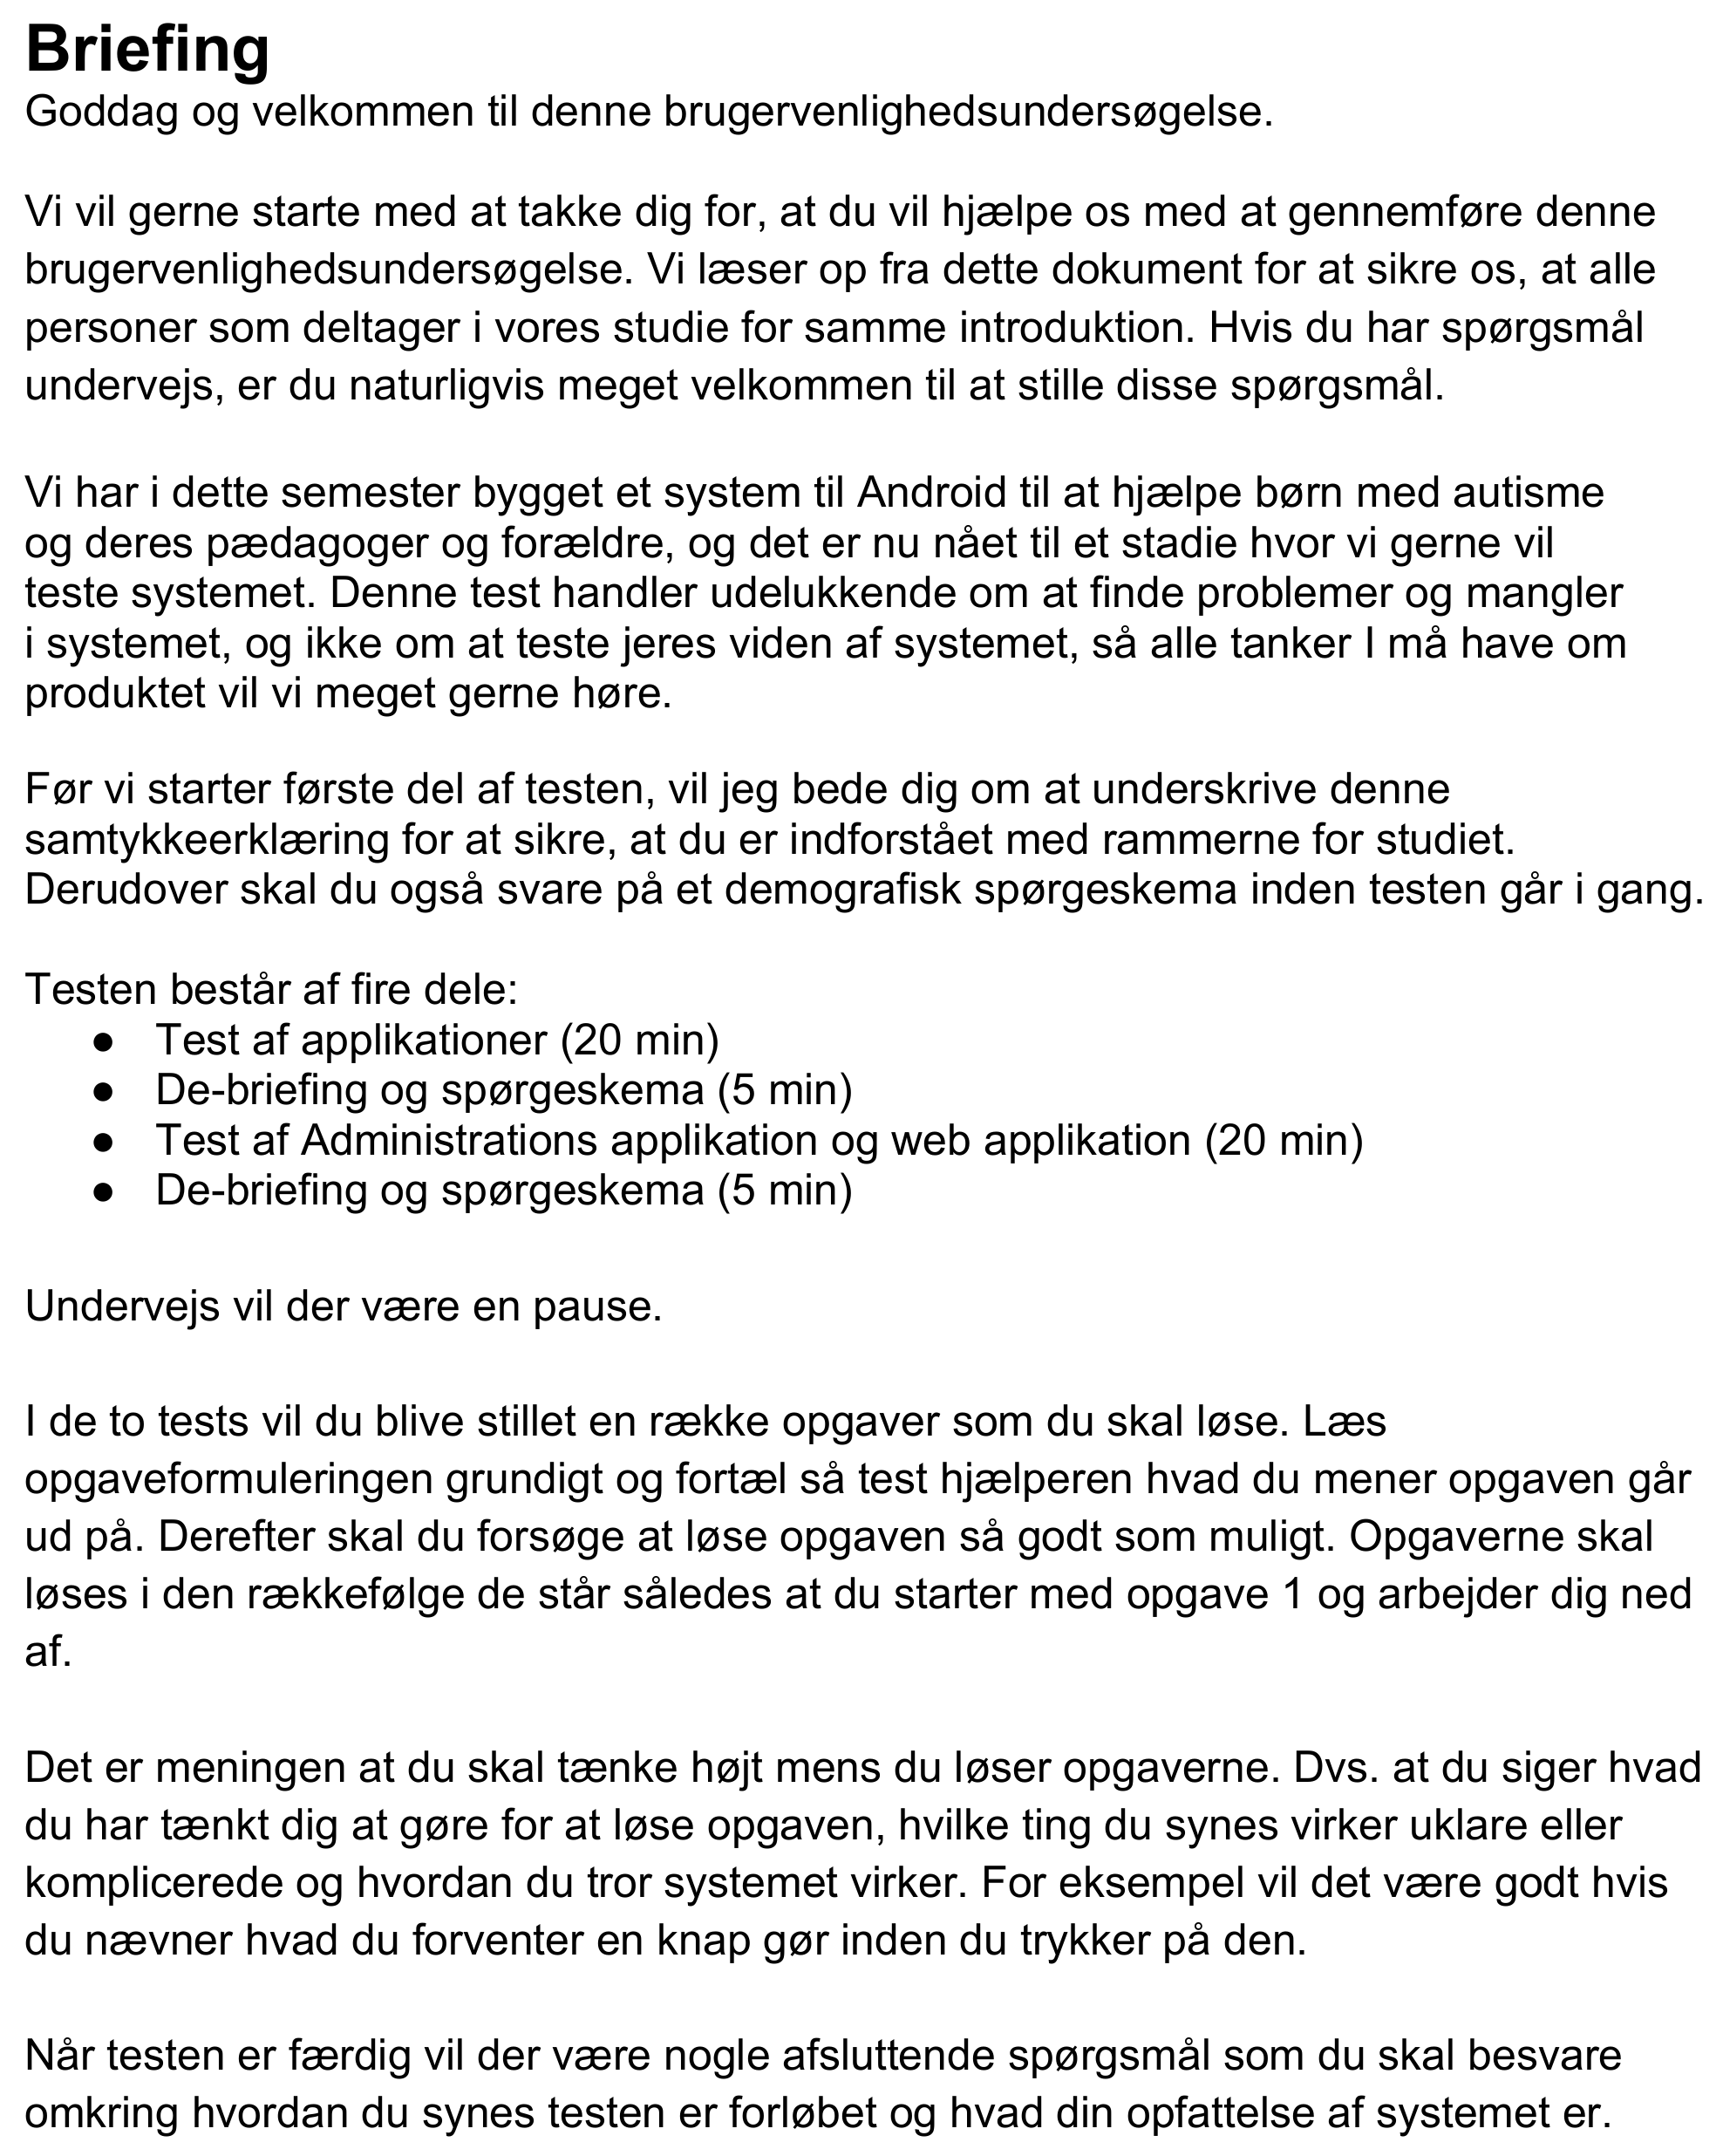
\includegraphics[scale=0.8]{gfx/usability-briefing.png}
	\caption{Briefing given to test subjects prior to testing}
	\label{fig:usability_briefing}
\end{figure}

\section{Demographic Questionnaire}
\begin{figure}[h!]
	\centering
	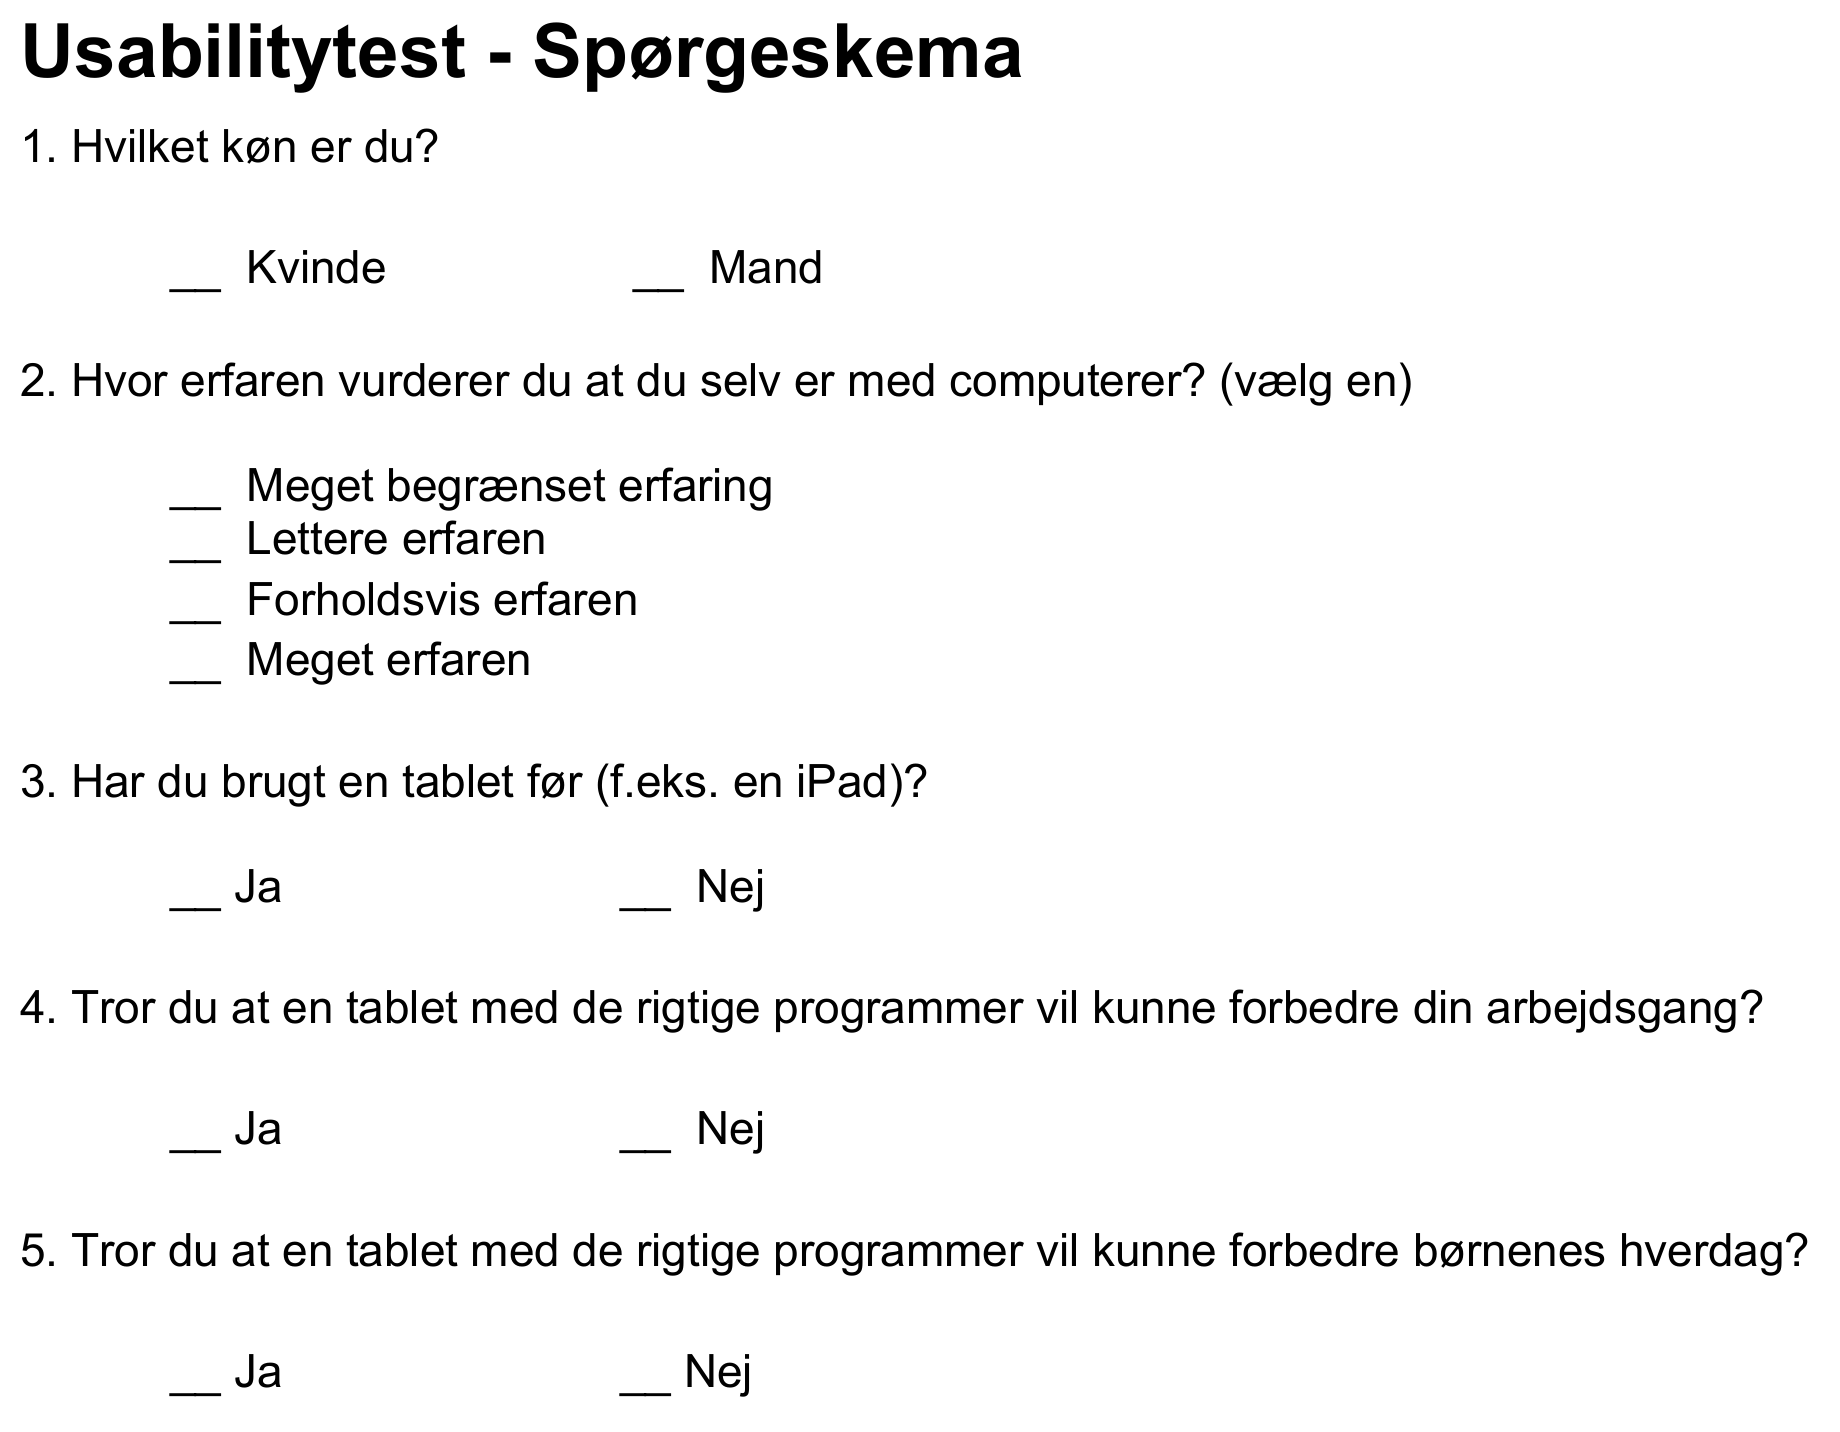
\includegraphics[scale=0.7]{gfx/usability-questionnaire.png}
	\caption{Demographic questionnaire filled out by the test subjects before the test. Afterwards, each subject was asked to rate the difficulty of each application on a five scale rating.}
	\label{fig:usability_questionnaire}
\end{figure}

\chapter{Test Cases}
\label{test_cases}
Overall requirements: \newline
Launcher is installed on a tablet running Android 3.2.x \newline

The tests are grouped based on the class they exist in, with the identifier of each test case being the name of the function tested and the number of the test for that function. \newline

For the second part of the tests of Tools-functions, the following apps must be present in the system as noted for each of them. \newline

WOMBAT (is a GIRAF app):
\begin{itemize}
\item is in the database.
\item is installed on the device.
\item is attached to the current user.
\end{itemize}

PARROT (GIRAF):
\begin{itemize}
\item is in the database.
\item is installed on the device.
\item is \textbf{not} attached to the current user.
\end{itemize}

ViewDB (GIRAF):
\begin{itemize}
\item is \textbf{not} in the database.
\item is installed on the device.
\item is \textbf{not} attached to the current user.
\end{itemize}

Lion (GIRAF):
\begin{itemize}
\item is in the database.
\item is \textbf{not} installed on the device.
\item is \textbf{not} attached to the current user.
\end{itemize}

Leopard (GIRAF):
\begin{itemize}
\item is in the database
\item is \textbf{not} installed on the device.
\item is attached to the current user.
\end{itemize}

Calculator (is an Android app):
\begin{itemize}
\item is in the database.
\item is installed on the device.
\item is attached to the current user.
\end{itemize}

Camera (Android):
\begin{itemize}
\item is in the database.
\item is installed on the device.
\item is \textbf{not} attached to the current user.
\end{itemize}

Gallery (Android):
\begin{itemize}
\item is \textbf{not} in the database.
\item is installed on the device.
\item is \textbf{not} attached to the current user.
\end{itemize}

Internet (Android):
\begin{itemize}
\item is in the database.
\item is \textbf{not} installed on the device.
\item is \textbf{not} attached to the current user.
\end{itemize}

Mail (Android):
\begin{itemize}
\item is in the database
\item is \textbf{not} installed on the device.
\item is attached to the current user.
\end{itemize}

\begin{table}[ht]
\caption{Test cases for the AppAdapter class} % title of Table
\centering  % used for centering table
\begin{tabular}{| p{1.7in} | p{1.7in} | p{1.7in} |}
\hline
Name: & Test: & Pass Criteria: \\ [0.5ex] % inserts table 
%heading
\hline                  % inserts single horizontal line
setAppBackground-001: & Call setAppBackground with the color 0xFFFFFFFF. & The background of the app is the color 0xFFFFFFFF. \\ \hline 
saveAppBackground-001: & Call saveAppBackground with the color 0xFFFFFFFF. & The launcher settings are changed so the color for the given app is 0xFFFFFFFF. \\ [1ex]      % [1ex] adds vertical space
\hline %inserts single line
\end{tabular}
\label{table:appadapter_tests} % is used to refer this table in the text
\end{table}

\begin{table}[ht]
\caption{Test cases for the AppInfo class} % title of Table
\centering  % used for centering table
\begin{tabular}{| p{1.7in} | p{1.7in} | p{1.7in} |}
\hline
Name: & Test: & Pass Criteria: \\ [0.5ex] % inserts table 
%heading
\hline    
setGuardian-001: & Call setGuardian with a non-guardian profile. & The guardian of the AppInfo is null. \\ \hline 
setGuardian-002: & Call setGuardian with a guardian profile. & The guardian of the AppInfo is the guardian used as input. \\ \hline
getShortenedName-001: & Call getShortenedName on an AppInfo with a name of five characters. & The return value is equal to the name of the AppInfo. \\ \hline 
getShortenedName-002: & Call getShortenedName on an AppInfo with a name of six characters. & The return value is equal to the name of the AppInfo. \\ \hline 
getShortenedName-003: & Call getShortenedName on an AppInfo with a name of seven characters. & The returned string consists of six characters with "`..."' concatinated. \\ [1ex] 
\hline %inserts single line
\end{tabular}
\label{table:appinfo_tests} % is used to refer this table in the text
\end{table}

\begin{table}[ht]
\caption{Test cases for the AuthenticationActivity class} % title of Table
\centering  % used for centering table
\begin{tabular}{| p{1.7in} | p{1.7in} | p{1.7in} |}
\hline
Name: & Test: & Pass Criteria: \\ [0.5ex] % inserts table 
%heading
\hline    
changeCamerafeed\newline{}BorderColor-001: & Scan an invalid QR code. & The camera feed border changes to red. \\ \hline 
changeCamerafeed\newline{}BorderColor-002: & Scan a valid QR code. & The camera feed border changes to green. \\ \hline
handleDecode-001: & Scan an invalid QR code. & The camera feed border changes to red and no log-in button and name is shown. \\ \hline 
handleDecode-002: & Scan a valid QR code. & The camera feed border changes to green, a log-in button appears, the name of the user attached to the QR code appears and the device vibrates. \\ [1ex] 
\hline %inserts single line
\end{tabular}
\label{table:authenticationactivity_tests} % is used to refer this table in the text
\end{table}

\begin{table}[ht]
\caption{Test cases for the HomeActivity class} % title of Table
\centering  % used for centering table
\begin{tabular}{| p{1.7in} | p{1.7in} | p{1.7in} |}
\hline
Name: & Test: & Pass Criteria: \\ [0.5ex] % inserts table 
%heading
\hline    
onBackPressed-001: & Press the device back button while on the home screen. & Nothing happens. \\ \hline 
calculateNumOfColumns-001: & The user should have nine apps visible to them. Call calculateNumOfCollumns(). & The returned number is four. \\ \hline
calculateNumOfColumns-002: & The user should have ten apps visible to them. Call calculateNumOfCollumns(). & The returned number is four. \\ \hline 
calculateNumOfColumns-003: & The user should have thirteen apps visible to them. Call calculateNumOfCollumns(). & The returned number is five. \\ \hline 
appBgColor-001: & A color for a given app already exists in the settings. Call appBgColor(). & The color returned matches the one from the settings. \\ \hline 
saveNewBgColor-001: & Call saveNewBgColor() with a real color and the ID of an app in the database. & This color has been saved in the settings. \\ \hline 
saveNewBgColor-002: & Call saveNewBgColor() with null as a color and the ID of an app in the database. & The settings are not changed. \\ \hline 
saveNewBgColor-003: & Call saveNewBgColor() with a real color and null as the ID. & The settings are not changed. \\ [1ex] 
\hline %inserts single line
\end{tabular}
\label{table:homeactivity_tests} % is used to refer this table in the text
\end{table}

\begin{table}[ht]
\caption{Test cases for the ProfileSelectActivity class} % title of Table
\centering  % used for centering table
\begin{tabular}{| p{1.7in} | p{1.7in} | p{1.7in} |}
\hline
Name: & Test: & Pass Criteria: \\ [0.5ex] % inserts table 
%heading
\hline                  % inserts single horizontal line
loadProfiles-001: & Call loadProfiles() for a guardian with children attached and different departments that also have children attached. & The returned list of children contains all children attached to the given guardian and the children attached to the departments of the guardian, but no duplicates. \\ [1ex]  
\hline %inserts single line
\end{tabular}
\label{table:profileselectactivity_tests} % is used to refer this table in the text
\end{table}

\begin{table}[ht]
\caption{Test cases for the Tools class, part one} % title of Table
\centering  % used for centering table
\begin{tabular}{| p{1.7in} | p{1.7in} | p{1.7in} |}
\hline
Name: & Test: & Pass Criteria: \\ [0.5ex] % inserts table 
%heading
\hline    
saveLogInData-001: & Login as an valid guardian. & The correct ID and timestamp is saved in shared preferences. \\ \hline 
findCurrentUser-001: & Call findCurrentUser(). & The currently logged in profile is returned. \\ \hline
findCurrentUserID-001: & Call findCurrentUserID(). & The currently correct profile ID is returned. \\ \hline 
clearAuthData-001: & Call clearAuthData(). & The ID is set to -1 and time to 1 in the shared preferences. \\ \hline 
sessionExpired-001: & Let the session to expire after 1 minute. \newline Log in as a valid guardian. Turn off device. Wait one minuted. Turn on device. & The guardian is logged out. \\ [1ex] 
\hline %inserts single line
\end{tabular}
\label{table:tools_tests1} % is used to refer this table in the text
\end{table}

\begin{table}[ht]
\caption{Test cases for the Tools class, part two (where the app requirements are enforced)} % title of Table
\centering  % used for centering table
\begin{tabular}{| p{1.7in} | p{1.7in} | p{1.7in} |}
\hline
Name: & Test: & Pass Criteria: \\ [0.5ex] % inserts table 
%heading
\hline    
getVisibleGirafApps-001: & Call getVisibleGirafApps() for the current user. & Only Wombat is returned. \\ \hline 
getVisibleAndroidApps-001: & Call getVisibleAndroidApps() for the current user. & Only Calculator is returned. \\ \hline
getVisibleApps-001: & Call getVisibleApps() for the current user. & Only Wombat and Calculator are returned. \\ \hline 
getHiddenGirafApps-001: & Call getHiddenGirafApps() for the current user. & Only Parrot is returned. \\ \hline 
getHiddenAndroidApps-001: & Call getHiddenAndroidApps() for the current user. & Only Camera is returned. \\ \hline 
getHiddenApps-001: & Call getHiddenApps() for the current user. & Only Parrot, ViewDB, Lion, Camera, Gallery and Internet are returned. \\ \hline 
getAvaliableGirafApps-001: & Call getAvaliableGirafApps() for the current user. & Only Wombat and Parrot are returned. \\ \hline 
getAvaliableAndroidApps-001: & Call getAvaliableAndroidApps() for the current user. & Only Calculator and Camera is returned. \\ \hline 
getAvaliableApps-001: & Call getAvaliableApps() for the current user. & Only Wombat, Parrot, Calculator and Camera is returned. \\ \hline 
getDeviceGirafApps-001: & Call getDeviceGirafApps() for the current user. & Verify that Wombat, Parrot and ViewDB is shown. \\ \hline 
getDeviceAndroidApps-001: & Call getDeviceAndroidApps() for the current user. & Only Calculator, Camera and Gallery is returned. \\ \hline 
getDeviceApps-001: & Call getDeviceApps() for the current user. & Only Wombat, Parrot, ViewDB, Calculator, Camera and Gallery is returned. \\ \hline 
subtractAppsList-001: & Call subtractAppsList with a[wombat,Calculator] and b[Calculator]. & Only Wombat is returned. \\ [1ex] 
\hline %inserts single line
\end{tabular}
\label{table:tools_tests2} % is used to refer this table in the text
\end{table}

\begin{table}[ht]
\centering  % used for centering table
\begin{tabular}{| p{1.7in} | p{1.7in} | p{1.7in} |}
\hline  
packageRegistered-001: & Call packageRegistered() with Wombat. & True is returned. \\ \hline 
packageRegistered-002: & Call packageRegistered() with ViewDB. & False is returned. \\ \hline 
insertAppInDB-001: & Call insertAppInDB() with ViewDB. & ViewDB is now in the database. \\ \hline 
attachLauncher-001: & A relation between the launcher and given user does not currently exist. Call attachLauncher() with the given user. & A relation between the launcher and user now exists in the database. \\ \hline 
appsContain\_{}RI-001: & Call appsContain\_{}RI with list of apps installed on the device as ResolveInfo's and Parrot. & True is returned. \\ \hline 
appsContain\_{}RI-002: & Call appsContain\_{}RI with list of apps installed on the device as ResolveInfo's and Lion. & False is returned. \\ \hline 
appsContain\_{}A-001: & Call appsContain\_{}A with a list of apps in the database and Wombat. & True is returned. \\ \hline 
appsContain\_{}A-002: & Call appsContain\_{}A with a list of apps in the database and ViewDB. & False is returned. \\ [1ex] 
\hline %inserts single line
\end{tabular}
\end{table}

\chapter{Authentication Design}
\label{app:design:authentication}
\begin{figure}[h!]
	\centering
	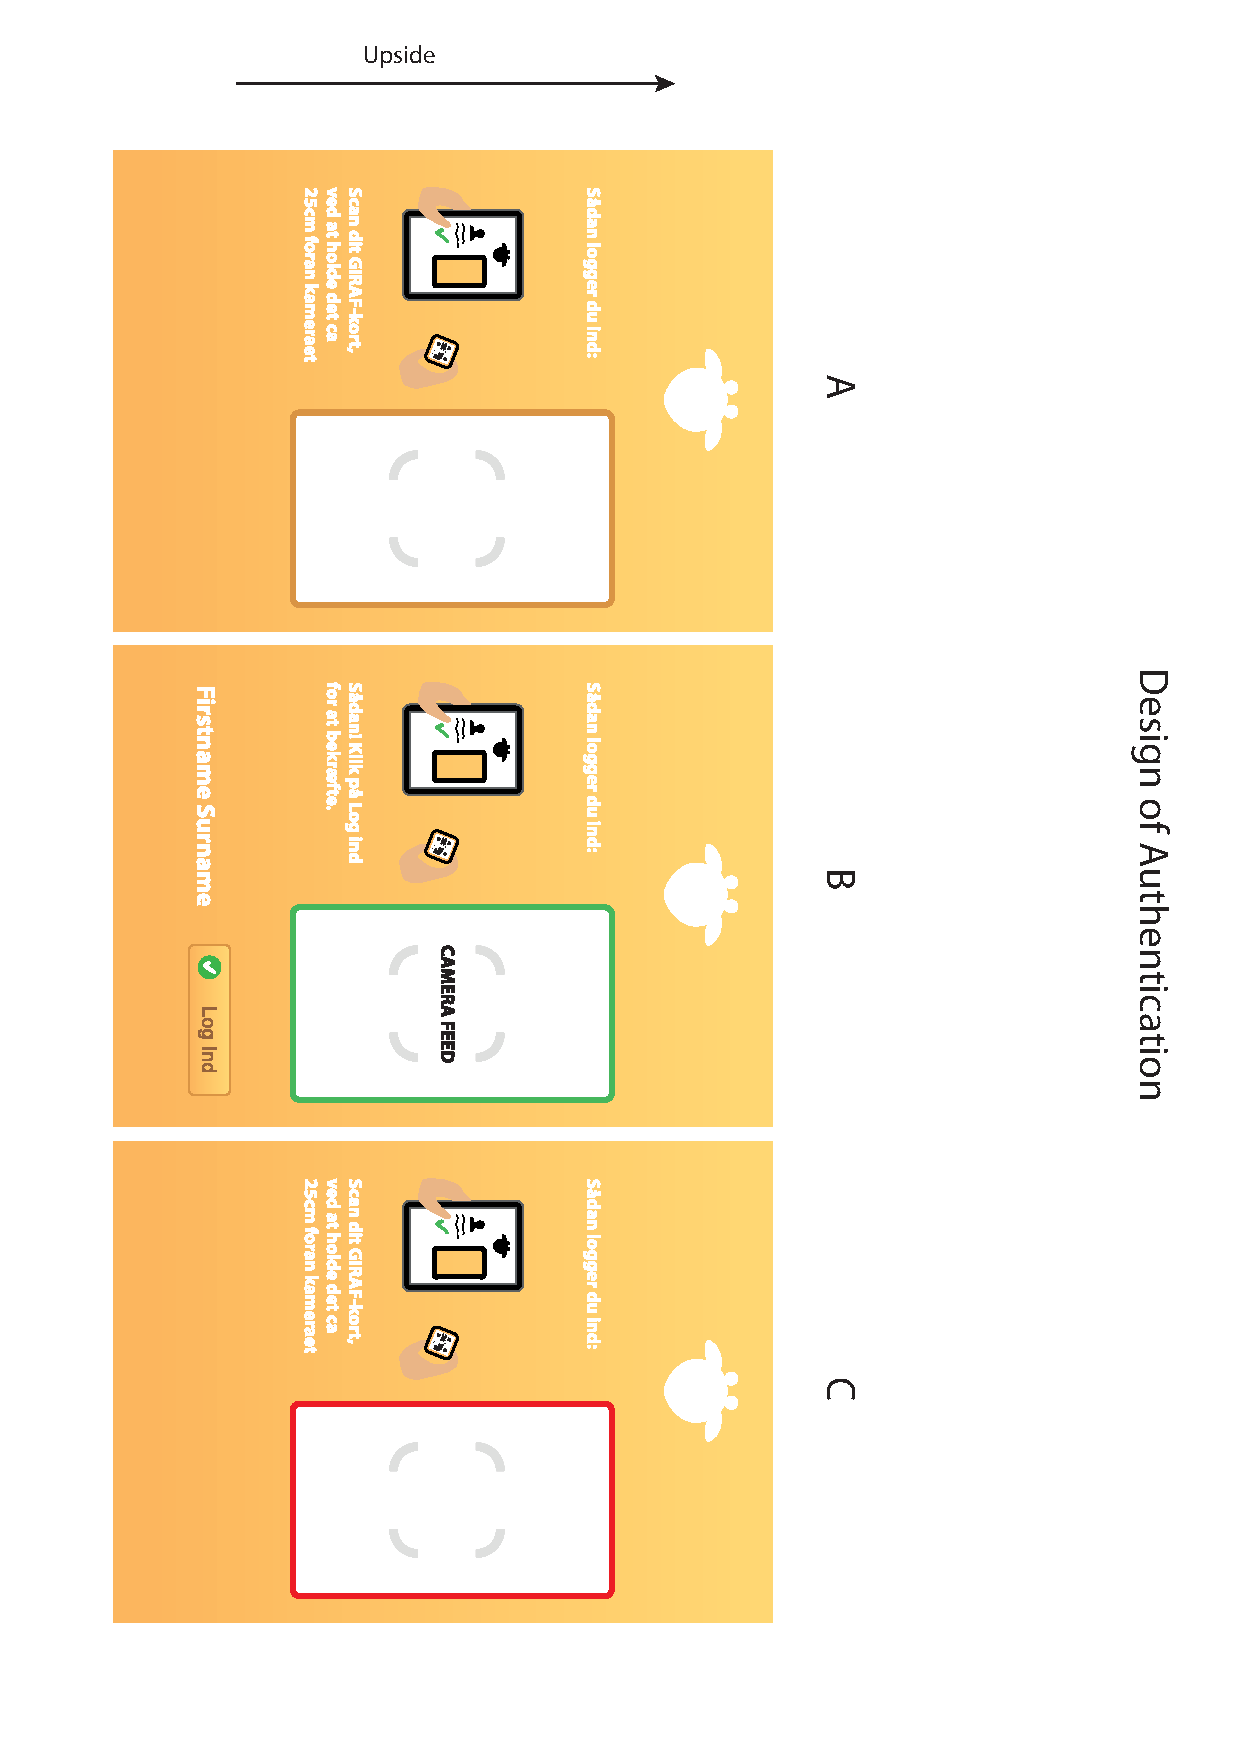
\includegraphics[width=\textwidth]{gfx/appendix_design_authentication.pdf}
	\caption{Authentication design}
	
\end{figure}

\chapter{\guicomponents[] Inheritance Trees}
\label{appendix:guiinheritance}

These trees show how the components in the \guicomponents[] library extends from each other. 

\begin{figure}[h]
	\centering
	\Tree [.BaseAdapter [.GColorAdapter ] GProfileAdapter ]
	\caption{Inheritance of \giraf[] adapters}
	\label{fig:gadapterinheritance}
\end{figure}

\begin{figure}[h]
	\centering
	\Tree [.Dialog [.GDialog ] GTooltip ]
	\caption{Inheritance of \giraf[] dialogs}
	\label{fig:gdialoginheritance}
\end{figure}

\begin{figure}[h]
	\centering
	\Tree [.ImageView [.GWidgetConnectivity ] GWidgetLogout ]
	\caption{Inheritance of \giraf[] ImageView}
	\label{fig:gimageviewinheritance}
\end{figure}

\begin{figure}[h]
	\centering
	\Tree [.TextView [.GWidgetCalendar ] ]
	\caption{Inheritance of \giraf[] TextView}
	\label{fig:gtextviewinheritance}
\end{figure}

\begin{figure}[h]
	\centering
	\Tree [.Handler [.GWidgetUpdater ] ]
	\caption{Inheritance of \giraf[] Handler}
	\label{fig:ghandlerinheritance}
\end{figure}

\begin{figure}[h]
 \centering
 \Tree [.ListView GList ]
 \caption{Inheritance of \giraf[] ListView}
 \label{fig:glistinheritance}
\end{figure}

\chapter{Launcher Services}
\label{appendix:launcherservices}
``Hvad vi stiller til r\aa{}dighed''\\

\textbf{Child ID} (v001) -- Det barn en app skal k\o{}res for f\aa{}r sit ID (en Long) sendt med i det Intent, der starter appen. For at f\aa{} fat i IDet skal f\o{}lgende g\o{}res inde i main activity:\\

	\verb+Long id = getIntent().getExtras().getLong(+``\verb+currentChildID+''\verb+);+\\
	
\textbf{Guardian ID} (v001) -- Den guardian, der starter en app f\aa{}r sit ID (en Long) sendt med i det Intent, der starter appen. For at f\aa{} fat i IDet skal f\o{}lgende g\o{}res inde i main activity:\\

	\verb+Long id = getIntent().getExtras().getLong(+``\verb+currentGuardianID+''\verb+);+\\
	
\textbf{Authentication} (v002) -- Vores QR authentication activity stilles til r\aa{}dighed, og kan kaldes med f\o{}lgende kode (den returnerer ikke data):\\

	\verb+Intent i = new Intent(+``\verb+dk.aau.cs.giraf.launcher.AUTHENTICATE+''\verb+);+
	\verb+i.addCategory(+``\verb+dk.aau.cs.giraf.launcher.GIRAF+''\verb+);+
	\verb+startActivity(i);+\\
	
OBS! Authentication h\aa{}ndterer ikke tryk p\aa{} Home- og Back-knapperne, og kan derfor nemt omg\aa{}s i den nuv\ae{}rende version. Vi har pt. ingen planer om at g\o{}re noget ved dette, s\aa{} mener man at den funktionalitet er vores ansvar er man velkommen til at komme ind og snakke med os om det.\\

\textbf{Background color} (v003) -- I launcheren har hver app en baggrund og farven p\aa{} den baggrund bliver sendt med i et intentet, der \aa{}bner apps. Hent det s\aa{}ledes:\\

\verb+int color = getIntent().getExtras().getInt(+``\verb+appBackgroundColor+''\verb+);+